\documentclass{article}
\usepackage[utf8]{inputenc}
\usepackage[T1]{fontenc}
\usepackage{graphicx}
\usepackage{amsmath, amssymb}
\usepackage{xcolor}
\usepackage{tikz}
\usepackage{lipsum}
\usepackage{enumerate}
\usepackage{sectsty}

\title{Practice Questions}
\author{Hia Al Saleh}
\date{February 20th, 2024}
\begin{document}
\maketitle
\section*{Chapter 1.2}
Page 26, \#1-7, 12, 13, 15, 16
\begin{itemize}
    \item Question 1: \\
    a) 4th degree polynomial \\
    b) 5th degree polynomial \\
    c) 4th degree polynomial \\
    d) 5th degree polynomial \\
    e) 2rd degree polynomial \\
    
    \item Question 2: \\
    a) postive \\
    b) quad 2 $\to$ 1 \\ 
    c) none \\ 
    d) 1 max, 2 min, local maximum one \\ 
    
    \item Question 3:\\
\textbf{a)} $f(x) = x^2 +3x- 1$
\begin{enumerate}
    \item[i)] End behavior: As $x$ approaches positive or negative infinity, $f(x)$ approaches positive infinity.
    \item[ii)] Constant finite differences: First finite differences.
    \item[iii)] Value of constant finite differences: $4$.
\end{enumerate}

\textbf{b)} $g(x) =-4x^3+ 2x^2 - x + 5$
\begin{enumerate}
    \item[i)] End behavior: As $x$ approaches positive infinity, $g(x)$ approaches negative infinity, and as $x$ approaches negative infinity, $g(x)$ approaches positive infinity.
    \item[ii)] Constant finite differences: Second finite differences.
    \item[iii)] Value of constant finite differences: $-6$.
\end{enumerate}

\textbf{c)} $h(x) = -7x^4 +2x^3 - 3x^2 + 4$
\begin{enumerate}
    \item[i)] End behavior: As $x$ approaches positive or negative infinity, $h(x)$ approaches negative infinity.
    \item[ii)] Constant finite differences: Third finite differences.
    \item[iii)] Value of constant finite differences: $0$.
\end{enumerate}

\textbf{d)} $p(x) = 0.6x^5 -2x^4 + 8x$
\begin{enumerate}
    \item[i)] End behavior: As $x$ approaches positive or negative infinity, $p(x)$ approaches positive infinity.
    \item[ii)] Constant finite differences: Fourth finite differences.
    \item[iii)] Value of constant finite differences: $7.2$.
\end{enumerate}

\textbf{e)} $f(x) = 3x$
\begin{enumerate}
    \item[i)] End behavior: As $x$ approaches positive or negative infinity, $f(x)$ approaches positive infinity.
    \item[ii)] Constant finite differences: First finite differences.
    \item[iii)] Value of constant finite differences: $3$.
\end{enumerate}

\textbf{f)} $h(x) = -x^6 + 8x^3$
\begin{enumerate}
    \item[i)] End behavior: As $x$ approaches positive infinity, $h(x)$ approaches negative infinity, and as $x$ approaches negative infinity, $h(x)$ approaches positive infinity.
    \item[ii)] Constant finite differences: Fifth finite differences.
    \item[iii)] Value of constant finite differences: $6$.
\end{enumerate}
    
    
\item Question 4:

\textbf{a)} Second differences = $-8$
\begin{enumerate}
    \item Degree of polynomial function: $2$ (quadratic)
    \item Leading coefficient: $\frac{-8}{2!} = -4$
\end{enumerate}

\textbf{b)} Fourth differences = $-48$
\begin{enumerate}
    \item Degree of polynomial function: $4$ (quartic)
    \item Leading coefficient: $\frac{-48}{4!} = -2$
\end{enumerate}

\textbf{c)} Third differences = $12$
\begin{enumerate}
    \item Degree of polynomial function: $3$ (cubic)
    \item Leading coefficient: $\frac{12}{3!} = 2$
\end{enumerate}

\textbf{d)} Fourth differences = $24$
\begin{enumerate}
    \item Degree of polynomial function: $4$ (quartic)
    \item Leading coefficient: $\frac{24}{4!} = 1$
\end{enumerate}

\textbf{e)} Third differences = $36$
\begin{enumerate}
    \item Degree of polynomial function: $3$ (cubic)
    \item Leading coefficient: $\frac{36}{3!} = 6$
\end{enumerate}

\textbf{f)} Fifth differences = $60$
\begin{enumerate}
    \item Degree of polynomial function: $5$ (quintic)
    \item Leading coefficient: $\frac{60}{5!} = 1$
\end{enumerate}

    \item Question 5
\begin{enumerate}[a)]
    \item Odd
    \item[b)] Even
    \item[c)] Odd
    \item[d)] Even
\end{enumerate}

    \item Question 6: \\
5a)
\begin{enumerate}[a)]
        \item 5 
        \item Negative 
        \item $2 \to 4$ 
        \item $x\to -\infty, y\to \infty\\ x\to \infty, y\to -\infty$ 
\end{enumerate}
5b)
\begin{enumerate}[a)]
        \item 4 
        \item Positive 
        \item $2 \to 1$ 
        \item $x\to -\infty, y\to \infty\\ x\to \infty, y\to \infty$ 
\end{enumerate}
5c)
\begin{enumerate}[a)]
        \item 3 
        \item Positive 
        \item $3 \to 1$ 
        \item $x\to -\infty, y\to \infty\\ x\to \infty, y\to \infty$ 
\end{enumerate}
\newpage 
5d)
\begin{enumerate}[a)]
        \item 6 
        \item Negative 
        \item $3 \to 4$ 
        \item $x\to -\infty, y\to \infty\\ x\to \infty, y\to -\infty$ 
\end{enumerate}
    
    \item Question 7: \\
    a)
    \begin{enumerate}[i)]
        \item 3
        \item Positive
        \item $6=a\cdot3!$\\ 1=a
    \end{enumerate}
    b)
    \begin{enumerate}[i)]
        \item 4
        \item Negative
        \item $24=a\cdot4!$\\ a=-1
    \end{enumerate}
    \item Question 12: \\
    \textbf{a)} The function $r(d)$ is a polynomial function.

\textbf{b)} Finite differences: The second finite differences will be constant for this function because the leading term of the function is $-0.7d^3$, which is a cubic term.

\textbf{c)} End behavior: As $d$ approaches positive or negative infinity, $r(d)$ will also approach positive infinity because the leading term of the function is $-0.7d^3$, which dominates the behavior of the function.

\textbf{d)} Restrictions: There might be restrictions on the amount of drug $d$ that can be administered to the patient. For instance, there could be a maximum safe dosage or a minimum effective dosage prescribed by medical guidelines or the physical limitations of the patient's body.
    \item Question 13: 
    \textbf{a)} Key features of the graph:
\begin{itemize}
    \item The function $p(t)$ is a quartic function.
    \item The leading term is $6t^4$, indicating that the function grows rapidly as $t$ increases or decreases without any restrictions.
    \item The function might have local maxima or minima depending on the values of the coefficients.
\end{itemize}

\textbf{b)} Constant finite differences: The fourth finite differences will be constant for this function because the leading term of the function is $6t^4$, which is a quartic term.

\textbf{c)} Current population: To find the current population of the town, plug in $t = 0$ into the function $p(t)$:
\[ p(0) = 6(0)^4 - 5(0)^3 + 200(0) + 12000 = 12000 \]
So, the current population of the town is $12,000$.

\textbf{d)} Population 10 years from now: To find the population of the town 10 years from now, plug in $t = 10$ into the function $p(t)$:
\[ p(10) = 6(10)^4 - 5(10)^3 + 200(10) + 12000 \]
\[ p(10) = 6(10000) - 5(1000) + 2000 + 12000 = 60000 - 5000 + 2000 + 12000 = 74000 \]
So, the population of the town 10 years from now will be $74,000$.

\textbf{e)} Time when population is approximately $175,000$: To find when the population of the town will be approximately $175,000$, set $p(t)$ equal to $175,000$ and solve for $t$:
\[ 6t^4 - 5t^3 + 200t + 12000 = 175000 \]
Solving this equation will give the approximate time when the population reaches $175,000$.
    \item Question 15:
    \textbf{a)} Quartic function with a negative leading coefficient and three x-intercepts:
\begin{center}
\begin{tikzpicture}
\draw[<->] (-1.5,0) -- (1.5,0) node[right] {$x$};
\draw[<->] (0,-2) -- (0,2) node[above] {$y$};
\draw[domain=-1:1, smooth, variable=\x, blue] plot ({\x}, {-0.5*\x^4 + \x^3 - 2*\x^2 + 1});
\node[circle,fill,inner sep=2pt,label=below:{$x_1$}] at (-1,0) {};
\node[circle,fill,inner sep=2pt,label=below:{$x_2$}] at (0,0) {};
\node[circle,fill,inner sep=2pt,label=below:{$x_3$}] at (1,0) {};
\end{tikzpicture}
\end{center}
\newpage
\textbf{b)} Cubic function with a positive leading coefficient and two x-intercepts:
\begin{center}
\begin{tikzpicture}
\draw[<->] (-1.5,0) -- (1.5,0) node[right] {$x$};
\draw[<->] (0,-2) -- (0,2) node[above] {$y$};
\draw[domain=-1:1, smooth, variable=\x, blue] plot ({\x}, {0.5*\x^3 - \x^2});
\node[circle,fill,inner sep=2pt,label=below:{$x_1$}] at (-1,0) {};
\node[circle,fill,inner sep=2pt,label=below:{$x_2$}] at (1,0) {};
\end{tikzpicture}
\end{center}

\textbf{c)} Quadratic function with a positive leading coefficient and no x-intercepts:
\begin{center}
\begin{tikzpicture}
\draw[<->] (-1.5,0) -- (1.5,0) node[right] {$x$};
\draw[<->] (0,-1) -- (0,2) node[above] {$y$};
\draw[domain=-1:1, smooth, variable=\x, blue] plot ({\x}, {0.5*\x^2 + 1});
\end{tikzpicture}
\end{center}

\textbf{d)} Quintic function with a negative leading coefficient and five x-intercepts:
\begin{center}
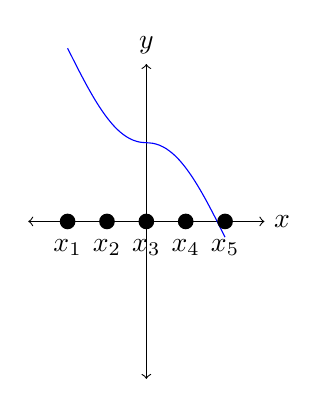
\begin{tikzpicture}
\draw[<->] (-1.5,0) -- (1.5,0) node[right] {$x$};
\draw[<->] (0,-2) -- (0,2) node[above] {$y$};
\draw[domain=-1:1, smooth, variable=\x, blue] plot ({\x}, {-0.2*\x^5 + \x^4 - \x^3 - \x^2 + 1});
\node[circle,fill,inner sep=2pt,label=below:{$x_1$}] at (-1,0) {};
\node[circle,fill,inner sep=2pt,label=below:{$x_2$}] at (-0.5,0) {};
\node[circle,fill,inner sep=2pt,label=below:{$x_3$}] at (0,0) {};
\node[circle,fill,inner sep=2pt,label=below:{$x_4$}] at (0.5,0) {};
\node[circle,fill,inner sep=2pt,label=below:{$x_5$}] at (1,0) {};
\end{tikzpicture}
\end{center}
\newpage
  \item Question 16
\textbf{a)} Possible numbers of x-intercepts for a quintic function: A quintic function can have up to 5 x-intercepts.

\textbf{b)} Sketch examples of a quintic function for each possibility in part a):
\begin{itemize}
    \item Quintic function with 0 x-intercepts:
    \begin{center}
    \begin{tikzpicture}
    \draw[<->] (-1.5,0) -- (1.5,0) node[right] {$x$};
    \draw[<->] (0,-1) -- (0,1) node[above] {$y$};
    \draw[domain=-1:1, smooth, variable=\x, blue] plot ({\x}, {0.1*\x^5 + 0.2*\x^4 - 0.3*\x^3 + 0.4*\x^2 - 0.5*\x + 0.1});
    \end{tikzpicture}
    \end{center}
    
    \item Quintic function with 1 x-intercept:
    \begin{center}
    \begin{tikzpicture}
    \draw[<->] (-1.5,0) -- (1.5,0) node[right] {$x$};
    \draw[<->] (0,-2) -- (0,2) node[above] {$y$};
    \draw[domain=-1:1, smooth, variable=\x, blue] plot ({\x}, {0.1*\x^5 + 0.2*\x^4 - 0.3*\x^3 + 0.4*\x^2 - 0.5*\x + 0.1});
    \node[circle,fill,inner sep=2pt,label=below:{$x_1$}] at (0,0) {};
    \end{tikzpicture}
    \end{center}
    
    \item Quintic function with 2 x-intercepts:
    \begin{center}
    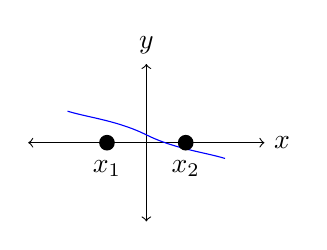
\begin{tikzpicture}
    \draw[<->] (-1.5,0) -- (1.5,0) node[right] {$x$};
    \draw[<->] (0,-1) -- (0,1) node[above] {$y$};
    \draw[domain=-1:1, smooth, variable=\x, blue] plot ({\x}, {-0.1*\x^5 + 0.2*\x^4 - 0.3*\x^3 + 0.4*\x^2 - 0.5*\x + 0.1});
    \node[circle,fill,inner sep=2pt,label=below:{$x_1$}] at (-0.5,0) {};
    \node[circle,fill,inner sep=2pt,label=below:{$x_2$}] at (0.5,0) {};
    \end{tikzpicture}
    \end{center}
    
    \item Quintic function with 3 x-intercepts:
    \begin{center}
    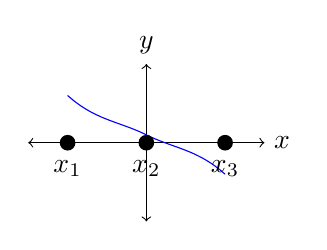
\begin{tikzpicture}
    \draw[<->] (-1.5,0) -- (1.5,0) node[right] {$x$};
    \draw[<->] (0,-1) -- (0,1) node[above] {$y$};
    \draw[domain=-1:1, smooth, variable=\x, blue] plot ({\x}, {0.1*\x^5 - 0.2*\x^4 - 0.3*\x^3 + 0.4*\x^2 - 0.5*\x + 0.1});
    \node[circle,fill,inner sep=2pt,label=below:{$x_1$}] at (-1,0) {};
    \node[circle,fill,inner sep=2pt,label=below:{$x_2$}] at (0,0) {};
    \node[circle,fill,inner sep=2pt,label=below:{$x_3$}] at (1,0) {};
    \end{tikzpicture}
    \end{center}
    \newpage
    \item Quintic function with 4 x-intercepts:
    \begin{center}
    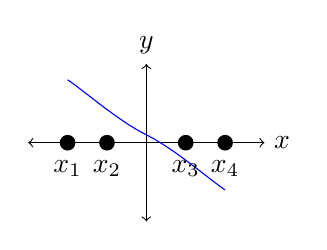
\begin{tikzpicture}
    \draw[<->] (-1.5,0) -- (1.5,0) node[right] {$x$};
    \draw[<->] (0,-1) -- (0,1) node[above] {$y$};
    \draw[domain=-1:1, smooth, variable=\x, blue] plot ({\x}, {0.1*\x^5 - 0.2*\x^4 + 0.3*\x^3 - 0.4*\x^2 - 0.5*\x + 0.1});
    \node[circle,fill,inner sep=2pt,label=below:{$x_1$}] at (-1,0) {};
    \node[circle,fill,inner sep=2pt,label=below:{$x_2$}] at (-0.5,0) {};
    \node[circle,fill,inner sep=2pt,label=below:{$x_3$}] at (0.5,0) {};
    \node[circle,fill,inner sep=2pt,label=below:{$x_4$}] at (1,0) {};
    \end{tikzpicture}
    \end{center}
    
    \item Quintic function with 5 x-intercepts:
    \begin{center}
    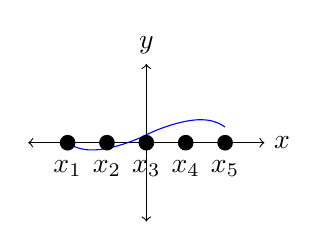
\begin{tikzpicture}
    \draw[<->] (-1.5,0) -- (1.5,0) node[right] {$x$};
    \draw[<->] (0,-1) -- (0,1) node[above] {$y$};
    \draw[domain=-1:1, smooth, variable=\x, blue] plot ({\x}, {-0.1*\x^5 - 0.2*\x^4 + 0.3*\x^3 - 0.4*\x^2 + 0.5*\x + 0.1});
    \node[circle,fill,inner sep=2pt,label=below:{$x_1$}] at (-1,0) {};
    \node[circle,fill,inner sep=2pt,label=below:{$x_2$}] at (-0.5,0) {};
    \node[circle,fill,inner sep=2pt,label=below:{$x_3$}] at (0,0) {};
    \node[circle,fill,inner sep=2pt,label=below:{$x_4$}] at (0.5,0) {};
    \node[circle,fill,inner sep=2pt,label=below:{$x_5$}] at (1,0) {};
    \end{tikzpicture}
    \end{center}
\end{itemize}
  
\end{itemize}
\end{document}
